\documentclass[11pt,a4paper]{article}

\usepackage[margin=2.5cm]{geometry}
\usepackage{booktabs}
\usepackage{longtable}
\usepackage{array}
\usepackage{hyperref}
\usepackage{xcolor}
\usepackage{tikz}
\usetikzlibrary{shapes.geometric, arrows.meta, positioning, fit, backgrounds}
\usepackage{parskip}
\usepackage{microtype}
\usepackage{caption}
\usepackage{amsmath}
\usepackage{enumitem}
\usepackage{tabularx}

\hypersetup{
  colorlinks=true,
  linkcolor=black,
  urlcolor=blue,
  citecolor=black
}

\definecolor{pipeblue}{RGB}{52, 120, 190}
\definecolor{pipegray}{RGB}{100, 100, 100}
\definecolor{pipegreen}{RGB}{40, 140, 80}

\title{\textbf{Supplementary Information}\\[0.5em]
  \large Automated Extraction of Experimental Parameters\\
  from the Public Goods Game Literature}
\author{}
\date{}

\begin{document}

\maketitle
\tableofcontents
\newpage

% ─────────────────────────────────────────────────────────────────────────────
\section{Overview}
\label{sec:overview}
% ─────────────────────────────────────────────────────────────────────────────

We developed a fully automated pipeline to extract structured experimental parameters from empirical papers on Public Goods Games (PGGs). The goal was to construct a machine-readable database of experimental conditions — one record per treatment arm — covering experimental design choices, independent and dependent variables, participant characteristics, and data provenance. The resulting dataset enables systematic comparisons across the PGG literature and serves as the empirical foundation for the prediction task described in the main paper.

The pipeline uses a large language model (LLM) to read each paper's full text in Markdown format and populate a predefined schema. Extraction is performed at the \emph{condition level}: if a paper reports four treatment arms (e.g.\ a 2×2 design), the pipeline produces four rows, one per arm. Field definitions, encoding rules, and worked examples are supplied in the prompt; the model is not asked to infer, impute, or extrapolate beyond what the paper explicitly states.

All code is available in the associated
\href{https://github.com/robin-na/LLM-literature-prediction}{GitHub repository}
(see \texttt{batch\_processing/}).

% ─────────────────────────────────────────────────────────────────────────────
\section{Corpus}
\label{sec:corpus}
% ─────────────────────────────────────────────────────────────────────────────

\subsection{Paper Selection}

The corpus consists of 810 papers identified through Web of Science searches for empirical and experimental PGG studies. Papers were selected based on title and abstract screening for relevance to the public goods contribution game paradigm, including variants with punishment, reward, communication, and other institutional mechanisms.

\subsection{Preparation}

Each paper was converted from PDF to Markdown (\texttt{.md}) format and stored in a shared Google Drive folder (\texttt{papers\_markdown}). The conversion preserves text, tables, and equations in a format the LLM can read directly. The script \texttt{download\_papers\_md.py} authenticates via OAuth 2.0 and downloads each file by matching the DOI-based filename. Files already present locally are skipped, making the download step idempotent.

\subsection{Scale}

\begin{itemize}[noitemsep]
  \item Papers submitted for extraction: 810
  \item Papers with at least one extractable experimental condition: 808
  \item Papers excluded (returned empty conditions): 2 — both were literature reviews or meta-analyses with no original experimental data
  \item Total condition rows extracted: 3{,}910
\end{itemize}

% ─────────────────────────────────────────────────────────────────────────────
\section{Extraction Pipeline}
\label{sec:pipeline}
% ─────────────────────────────────────────────────────────────────────────────

\subsection{Architecture}

Figure~\ref{fig:pipeline} illustrates the end-to-end extraction workflow.

\begin{figure}[h!]
\centering
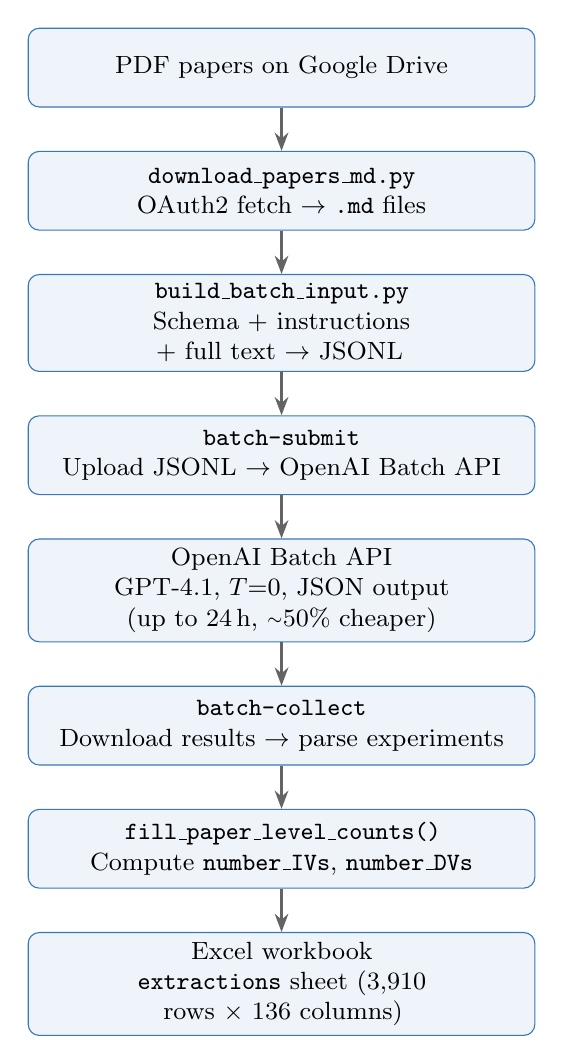
\begin{tikzpicture}[
  node distance = 0.55cm and 0cm,
  box/.style = {rectangle, rounded corners=4pt, draw=pipeblue, fill=pipeblue!8,
                text width=6.2cm, minimum height=1.0cm, align=center,
                font=\small},
  arrow/.style = {-Stealth, thick, color=pipegray},
  label/.style = {font=\footnotesize\itshape, color=pipegray, text width=4cm, align=left}
]

\node[box] (drive)   {PDF papers on Google Drive};
\node[box, below=of drive]  (dl)     {\texttt{download\_papers\_md.py}\\OAuth2 fetch $\to$ \texttt{.md} files};
\node[box, below=of dl]     (build)  {\texttt{build\_batch\_input.py}\\Schema + instructions + full text $\to$ JSONL};
\node[box, below=of build]  (submit) {\texttt{batch-submit}\\Upload JSONL $\to$ OpenAI Batch API};
\node[box, below=of submit] (oai)    {OpenAI Batch API\\GPT-4.1, $T{=}0$, JSON output\\(up to 24\,h, {\raise.17ex\hbox{$\scriptstyle\sim$}}50\% cheaper)};
\node[box, below=of oai]    (collect){\texttt{batch-collect}\\Download results $\to$ parse experiments};
\node[box, below=of collect](post)   {\texttt{fill\_paper\_level\_counts()}\\Compute \texttt{number\_IVs}, \texttt{number\_DVs}};
\node[box, below=of post]   (xlsx)   {Excel workbook\\\texttt{extractions} sheet (3{,}910 rows $\times$ 136 columns)};

\draw[arrow] (drive)   -- (dl);
\draw[arrow] (dl)      -- (build);
\draw[arrow] (build)   -- (submit);
\draw[arrow] (submit)  -- (oai);
\draw[arrow] (oai)     -- (collect);
\draw[arrow] (collect) -- (post);
\draw[arrow] (post)    -- (xlsx);

\end{tikzpicture}
\caption{End-to-end extraction pipeline. Each box corresponds to a discrete processing step. The OpenAI Batch API processes all 810 papers asynchronously; results are collected once all jobs are complete.}
\label{fig:pipeline}
\end{figure}

\subsection{Model and API}

Extraction uses \textbf{GPT-4.1} (OpenAI) at temperature 0 to ensure deterministic output. All requests are submitted via the \textbf{OpenAI Batch API} (\texttt{/v1/responses} endpoint with \texttt{response\_format: \{type: json\_object\}}), which processes jobs asynchronously at approximately 50\% of the real-time API cost and returns results within 24 hours.

Each request consists of:
\begin{enumerate}[noitemsep]
  \item A \textbf{system prompt} specifying the extraction role and JSON output constraint.
  \item A \textbf{user prompt} comprising (a) the output schema definition, (b) field-by-field instructions and worked examples, and (c) the full paper text.
\end{enumerate}

\subsection{Prompt Design}

\paragraph{Non-inference rule.}
The instruction set opens with a strict non-inference rule:
\begin{quote}
\textit{``Only report a value when the paper explicitly states it or when it is directly and unambiguously computable from reported numbers. Do NOT infer values from silence, convention, or reasonable assumption.''}
\end{quote}
This prevents the model from filling in plausible but unverified values based on domain conventions.

\paragraph{N/A versus N/R.}
Two sentinel values distinguish different types of missingness:
\begin{itemize}[noitemsep]
  \item \textbf{N/A} — the field is not applicable to this condition (e.g.\ \texttt{CONFIG\_punishmentCost} when no punishment mechanism exists).
  \item \textbf{N/R} — the field is applicable but the paper does not report the value.
\end{itemize}
Coding rules specify which sentinel to use for each field, preventing false zeros.

\paragraph{Condition-level instruction.}
The model is instructed to produce one JSON object per experimental condition within the \texttt{experiments} array. Papers with multi-arm designs produce multiple objects; single-condition papers produce one.

\paragraph{Reason and confidence.}
For each field \texttt{X}, the model also returns \texttt{X\_reason} (a brief justification quoting or paraphrasing the paper) and \texttt{X\_confidence} (a self-assessed numeric confidence on 0–1). These audit columns facilitate quality review.

% ─────────────────────────────────────────────────────────────────────────────
\section{Extraction Schema}
\label{sec:schema}
% ─────────────────────────────────────────────────────────────────────────────

The schema comprises 45 fields organised into five groups. The complete output has 136 columns per row: \texttt{custom\_id} plus three columns per field (value, reason, confidence). Table~\ref{tab:schema} lists all fields with their type, granularity, and definition.

\paragraph{Granularity notation.} \textit{Condition} fields may differ across treatment arms within a paper. \textit{Paper} fields take the same value for every row belonging to the same paper; they are computed or extracted once and propagated.

\renewcommand{\arraystretch}{1.35}
\begin{longtable}{p{3.9cm} p{1.2cm} p{2.1cm} >{\raggedright\arraybackslash}p{6.4cm}}
\caption{Complete extraction schema. Fields marked \dag{} are computed programmatically after LLM extraction (not asked to the model).}
\label{tab:schema}\\
\toprule
\textbf{Field} & \textbf{Type} & \textbf{Granularity} & \textbf{Definition} \\
\midrule
\endfirsthead
\multicolumn{4}{c}{\small\itshape Table \ref{tab:schema} continued}\\
\toprule
\textbf{Field} & \textbf{Type} & \textbf{Granularity} & \textbf{Definition} \\
\midrule
\endhead
\midrule
\multicolumn{4}{r}{\small\itshape Continued on next page}\\
\endfoot
\bottomrule
\endlastfoot

% ── Condition identification ──────────────────────────────────────────────────
\multicolumn{4}{l}{\textbf{Condition Identification}}\\[2pt]
\texttt{data\_id} & string & condition & Label the paper uses for this condition (e.g.\ ``Experiment 1 – Punishment Treatment'') \\
\texttt{indep\_var} & string & condition & Independent variable(s) and their value(s) for this row \\[4pt]

% ── Method ───────────────────────────────────────────────────────────────────
\multicolumn{4}{l}{\textbf{Method Classification}}\\[2pt]
\texttt{METHOD\_empirical} & bool & condition & True if the study uses human participants \\
\texttt{METHOD\_experiment} & bool & condition & True if controlled experiment; false if observational \\
\texttt{METHOD\_lab} & bool & condition & True if lab-based; false if field experiment \\
\texttt{METHOD\_simulation} & bool & condition & True if agent-based / computer simulation with no human subjects \\
\texttt{METHOD\_analytical} & bool & condition & True if formal mathematical model (no human subjects) \\[4pt]

% ── Config ───────────────────────────────────────────────────────────────────
\multicolumn{4}{l}{\textbf{Experimental Configuration}}\\[2pt]
\texttt{CONFIG\_playerCount} & int & condition & Number of strategic players per group. Teams count as one player; session headcount is not reported. \\
\texttt{CONFIG\_numRounds} & int & condition & Number of game rounds or periods \\
\texttt{CONFIG\_allOrNothing} & 0/1 & condition & 1 = continuous contribution choice (any amount 0–endowment); 0 = binary all-or-nothing contribution. N/A if not described. \textit{Note: the field name is counterintuitive; 1 denotes the more flexible, continuous case.} \\
\texttt{CONFIG\_defaultContribProp} & 0–1 & condition & Fraction of endowment placed in the public fund by default. 0 = standard VCM (private account default); 1 = opt-out game. N/A if not stated. \\
\texttt{CONFIG\_MPCR} & float & condition & Marginal per-capita return: group multiplier divided by group size \\
\texttt{CONFIG\_chat} & 0/1 & condition & 1 = unrestricted free-form communication explicitly permitted; 0 = explicitly prohibited; N/A if not mentioned \\
\texttt{CONFIG\_showOtherSummaries} & 0/1 & condition & 1 = participants receive post-round feedback on others' contributions or earnings; N/A if not mentioned \\
\texttt{CONFIG\_showPunishmentId} & 0/1 & condition & 1 = punished player can identify the punisher; 0 = anonymous punishment; N/A if no punishment or not stated \\
\texttt{CONFIG\_showRewardId} & 0/1 & condition & 1 = reward recipient can identify the rewarder; N/A if no reward or not stated \\
\texttt{CONFIG\_showNRounds} & 0/1 & condition & 1 only if paper explicitly states the round count or remaining rounds are displayed to participants. N/A if not stated — never coded 0 from silence. \\
\texttt{CONFIG\_punishmentExists} & 0/1 & condition & 1 only if a punishment mechanism is explicitly described for this condition; N/A if not mentioned \\
\texttt{CONFIG\_punishmentCost} & float & condition & Tokens spent by the punisher per unit of punishment assigned. N/A if no punishment. \\
\texttt{CONFIG\_punishmentTech} & float & condition & Reduction in target's payoff per unit of punishment received (the ``effectiveness'' ratio). N/A if no punishment. \\
\texttt{CONFIG\_rewardExists} & 0/1 & condition & 1 only if a reward mechanism is explicitly described; N/A if not mentioned \\
\texttt{CONFIG\_rewardCost} & float & condition & Tokens spent by the rewarder per unit of reward. N/A if no reward. \\
\texttt{CONFIG\_rewardTech} & float & condition & Increase in recipient's payoff per unit of reward received. N/A if no reward. \\
\texttt{CONFIG\_endowment} & float & condition & Initial token allocation per player per round \\[4pt]

% ── IV / DV ──────────────────────────────────────────────────────────────────
\multicolumn{4}{l}{\textbf{Independent and Dependent Variables}}\\[2pt]
\texttt{IVs} & JSON array & condition & Snake\_case names of experimental factors varied across conditions in this paper. Fixed parameters (e.g.\ endowment when constant across arms) are excluded. Example: \texttt{["punishment\_mechanism", "group\_size"]}. \\
\texttt{number\_IVs}\,\dag & int & paper & Count of unique IV names across all conditions in the paper, computed as $|\bigcup_{\text{conditions}} \texttt{IVs}|$. Same value in every row for a given paper. \\
\texttt{DVs} & JSON array & condition & Snake\_case names of outcome measures reported or analyzed for this specific condition. Conditions without punishment do not list punishment-related DVs. Example: \texttt{["individual\_contribution",\,"efficiency"]}. \\
\texttt{DVs\_Definitions} & JSON object & condition & Maps each DV name to its paper-specific definition. Keys must match the \texttt{DVs} array exactly. \\
\texttt{number\_DVs}\,\dag & int & paper & Count of unique DV names across all conditions in the paper, computed as $|\bigcup_{\text{conditions}} \texttt{DVs}|$. Same value in every row. \\
\texttt{DV\_efficiencyReported} & 0/1 & paper & 1 if efficiency (actual group payoff / maximum cooperative payoff) is reported anywhere in the paper; 0 only if it never appears. Same value in every row. \\[4pt]

% ── Study context ─────────────────────────────────────────────────────────────
\multicolumn{4}{l}{\textbf{Study Context}}\\[2pt]
\texttt{source\_data} & string & paper & \texttt{"Internal"}: data collected by the authors for this study (lab, online, or field). \texttt{"External"}: data borrowed from another experiment or archival dataset (reanalysis). Same value in every row. \\
\texttt{participant\_country} & string & condition & Country where the experiment was conducted. N/R if not stated. \\
\texttt{participant\_age} & string & condition & Age descriptor (e.g.\ ``student'', ``18--35 years''). N/R if not stated. \\
\texttt{participant\_gender} & string & condition & Gender composition: ``mixed'', ``male only'', ``female only'', or N/R. \\
\texttt{participant\_education} & string & condition & Education level (e.g.\ ``undergraduate students'', ``general population''). N/R if not stated. \\
\texttt{experiment\_environment} & categ. & condition & One of: \texttt{Online}, \texttt{On site}, \texttt{Field experiment}, \texttt{Observational}, \texttt{No human} \\
\texttt{other\_game\_info} & string & condition & Free-text field for additional design details not captured by other fields \\

\end{longtable}
\renewcommand{\arraystretch}{1.0}

% ─────────────────────────────────────────────────────────────────────────────
\section{Post-Processing}
\label{sec:postprocessing}
% ─────────────────────────────────────────────────────────────────────────────

Two fields — \texttt{number\_IVs} and \texttt{number\_DVs} — are computed programmatically after LLM extraction rather than being asked of the model directly. This design choice avoids a systematic LLM error in which models count \emph{levels} within a variable rather than unique variable \emph{names} (e.g.\ treating the binary variable ``punishment: yes/no'' as two independent variables rather than one).

The computation is performed by \texttt{fill\_paper\_level\_counts()} in \texttt{extraction\_pipeline.py}:

\begin{enumerate}[noitemsep]
  \item All condition rows for a paper are grouped by paper identifier (\texttt{custom\_id}).
  \item For each paper, the \texttt{IVs} and \texttt{DVs} JSON arrays are parsed from every condition row.
  \item The union of all IV names and the union of all DV names are accumulated into sets:
    \[
      \texttt{number\_IVs} = \left|\bigcup_{\text{conditions}} \texttt{IVs}_{\text{condition}}\right|, \quad
      \texttt{number\_DVs} = \left|\bigcup_{\text{conditions}} \texttt{DVs}_{\text{condition}}\right|
    \]
  \item The computed integer is written to every row of that paper (paper-level field).
\end{enumerate}

The union-based approach correctly handles designs in which some DVs appear only in specific conditions (e.g.\ punishment-related outcomes appear only in punishment arms): such DVs are included in the paper-level count because they appear in at least one condition.

% ─────────────────────────────────────────────────────────────────────────────
\section{Quality and Scale}
\label{sec:quality}
% ─────────────────────────────────────────────────────────────────────────────

\subsection{Extraction Results}

\begin{table}[h!]
\centering
\begin{tabular}{lr}
\toprule
\textbf{Metric} & \textbf{Value} \\
\midrule
Papers submitted & 810 \\
Papers with extractable conditions & 808 \\
Papers returning empty conditions & 2 \\
Total condition rows & 3{,}910 \\
Fields per condition & 45 \\
Output columns per row & 136 \\
\midrule
\texttt{source\_data = Internal} & 3{,}862 rows (98.8\%) \\
\texttt{source\_data = External} & 48 rows (1.2\%) \\
\bottomrule
\end{tabular}
\caption{Summary statistics for the extracted dataset.}
\label{tab:stats}
\end{table}

\subsection{Papers Excluded}

Two papers returned \texttt{\{"experiments": []\}}. Manual inspection confirmed both are literature reviews or meta-analyses that synthesise prior results without reporting original experimental data; they contain no conditions to extract. No extraction errors occurred.

\subsection{Output File}

The extracted dataset is stored in \texttt{batch\_processing/output\_xlsx/simple\_batch\_810papers.xlsx}, sheet \texttt{extractions}. Each row corresponds to one experimental condition; each field has three associated columns (value, reason, confidence score). Arrays (\texttt{IVs}, \texttt{DVs}) and dictionaries (\texttt{DVs\_Definitions}) are stored as JSON strings.

% ─────────────────────────────────────────────────────────────────────────────
\section{Reproducibility}
\label{sec:reproducibility}
% ─────────────────────────────────────────────────────────────────────────────

The extraction can be reproduced by following these steps:

\begin{enumerate}
  \item \textbf{Obtain papers.} Download Markdown files from Google Drive using \texttt{download\_papers\_md.py} with the PDF path list \texttt{batch\_processing/inputs/pdf\_paths\_800.txt}.

  \item \textbf{Submit batch job.}
\begin{verbatim}
python batch_processing/extract_papers.py batch-submit \
  --paper-dir PGG_papers/papers \
  --paper-ids $(cat batch_processing/inputs/paper_ids_800.txt \
                | tr '\n' ' ') \
  --model gpt-4.1 \
  --save-jsonl batch_processing/inputs/batch_input_810papers.jsonl
\end{verbatim}

  \item \textbf{Collect results} (once the batch status reports \texttt{completed}).
\begin{verbatim}
python batch_processing/extract_papers.py batch-collect <batch_id> \
  --output-xlsx \
    batch_processing/output_xlsx/simple_batch_810papers.xlsx \
  --save-jsonl \
    batch_processing/inputs/batch_output_810papers.jsonl
\end{verbatim}
\end{enumerate}

\noindent The raw batch output JSONL (\texttt{batch\_output\_810papers.jsonl}) is retained alongside the Excel file for full traceability.

\end{document}
